%%%%%%%%%%%%%%%%%%%%%%%%%%%%%%%%%%%%%%%%%
% Journal Article
% LaTeX Template
% Version 1.4 (15/5/16)
%
% This template has been downloaded from:
% http://www.LaTeXTemplates.com
%
% Original author:
% Frits Wenneker (http://www.howtotex.com) with extensive modifications by
% Vel (vel@LaTeXTemplates.com)
%
% License:
% CC BY-NC-SA 3.0 (http://creativecommons.org/licenses/by-nc-sa/3.0/)
%
%%%%%%%%%%%%%%%%%%%%%%%%%%%%%%%%%%%%%%%%%

%----------------------------------------------------------------------------------------
%	PACKAGES AND OTHER DOCUMENT CONFIGURATIONS
%----------------------------------------------------------------------------------------

\documentclass[twoside,twocolumn]{article}

\usepackage{blindtext} % Package to generate dummy text throughout this template 

\usepackage[sc]{mathpazo} % Use the Palatino font
\usepackage[T1]{fontenc} % Use 8-bit encoding that has 256 glyphs
\linespread{1.05} % Line spacing - Palatino needs more space between lines
\usepackage{microtype} % Slightly tweak font spacing for aesthetics

\usepackage[english]{babel} % Language hyphenation and typographical rules

\usepackage[hmarginratio=1:1,top=30mm,columnsep=18pt]{geometry} % Document margins
\usepackage[hang, small,labelfont=bf,up,textfont=it,up]{caption} % Custom captions under/above floats in tables or figures
\usepackage{booktabs} % Horizontal rules in tables

\usepackage{lettrine} % The lettrine is the first enlarged letter at the beginning of the text

\usepackage{enumitem} % Customized lists
\setlist[itemize]{noitemsep} % Make itemize lists more compact

\usepackage{abstract} % Allows abstract customization
\renewcommand{\abstractnamefont}{\normalfont\bfseries} % Set the "Abstract" text to bold
\renewcommand{\abstracttextfont}{\normalfont\small\itshape} % Set the abstract itself to small italic text

\usepackage{titlesec} % Allows customization of titles
\renewcommand\thesection{\Roman{section}} % Roman numerals for the sections
\renewcommand\thesubsection{\roman{subsection}} % roman numerals for subsections
\titleformat{\section}[block]{\large\scshape\centering}{\thesection.}{1em}{} % Change the look of the section titles
\titleformat{\subsection}[block]{\large}{\thesubsection.}{1em}{} % Change the look of the section titles

\usepackage{fancyhdr} % Headers and footers
\pagestyle{fancy} % All pages have headers and footers
\fancyhead{} % Blank out the default header
\fancyfoot{} % Blank out the default footer
\fancyhead[C]{Dennis Goldschmidt $\bullet$ Rotation report} % Custom header text
\fancyfoot[RO,LE]{\thepage} % Custom footer text

\usepackage{titling} % Customizing the title section
\usepackage{amsmath}
\usepackage{amssymb}
\usepackage{amsbsy}
\usepackage{hyperref} % For hyperlinks in the PDF
\usepackage{graphicx}% http://ctan.org/pkg/graphicx
\bibliographystyle{unsrtnat}
\usepackage[numbers,sort&compress]{natbib}

\renewcommand{\b}[1]{\textbf{#1}}
\newcommand{\tn}[1]{\textnormal{#1}}
\newcommand{\R}{\mathbb{R}}
\newcommand{\spaner}{\textnormal{span}}

%----------------------------------------------------------------------------------------
%	TITLE SECTION
%----------------------------------------------------------------------------------------

\setlength{\droptitle}{-4\baselineskip} % Move the title up

\pretitle{\begin{center}\Huge\bfseries} % Article title formatting
\posttitle{\end{center}} % Article title closing formatting
\title{\Large {Interactions of optimal balance and recurrent plasticity for compensating neuronal death} \\[0.25cm] \small{Machens lab rotation report}} % Article title
\author{%
\textsc{Dennis Goldschmidt} \\[1ex] % Your name
\normalsize Champalimaud Neuroscience Programme,  \\ % Your institution
\normalsize \href{mailto:dennis.goldschmidt@neuro.fchampalimaud.org}{dennis.goldschmidt@neuro.fchampalimaud.org} % Your email address
%\and % Uncomment if 2 authors are required, duplicate these 4 lines if more
%\textsc{Jane Smith}\thanks{Corresponding author} \\[1ex] % Second author's name
%\normalsize University of Utah \\ % Second author's institution
%\normalsize \href{mailto:jane@smith.com}{jane@smith.com} % Second author's email address
}
\date{\today} % Leave empty to omit a date
\renewcommand{\maketitlehookd}{%
\begin{abstract}
\noindent Information processing in the brain is surprisingly robust, even when facing neuronal death due to damaging environmental influences, neuronal aging, or neurodegenerative diseases. Many studies have shown that the robustness is due to adaptive molecular mechanisms and synaptic plasticity, which reorganize network connectivity. However, it is also hypothesized that neurons are able to self-regulate their firing properties to compensate for such perturbations. The theoretical framework of optimal balanced networks recently proposed a mechanism for such neuronal self-regulation based on quadratic optimization. This report describes simulations of optimal balanced networks to examine the interactions of firing rate compensation and recurrent plasticity during neuronal death. We find that after the rapid compensation by locally increased firing rates, recurrent plasticity can further recover the network's balance by decreasing the variance of the population rate. This leads to a lower coding error, especially for severe loss of more than 60\% of the population.  % Dummy abstract text - replace \blindtext with your abstract text
\end{abstract}
}

%----------------------------------------------------------------------------------------

\begin{document}

% Print the title
\maketitle

%----------------------------------------------------------------------------------------
%	ARTICLE CONTENTS
%\tableofcontents
%----------------------------------------------------------------------------------------

\section{Introduction}

The brain encodes and processes sensory stimuli in order to extract relevant information from the environment to act upon. Computational neuroscience is interested in finding out about the computational and algorithmic implementations of sensory information processing in the brain \cite{Marr1982}. Given that neurons transmit action potentials, it is apparent to ask how information might be represented in such a spike code. Early seminal works by Adrian \cite{Adrian1926} have shown that the firing rate of single neurons conveys information about the amplitude of a stimulus. However, the world contains an enormous amount of information continuously sensed by the sensory afferents and it also possesses a certain amount of uncertainty not only in stimuli, but also in actions generated by the brain. Nonetheless, brains are capable of processing this uncertain information and make appropriate decisions \cite{Ernst2002, Behrens2007, Drugowitsch2014}.  

Natural stimuli are spatially and temporally correlated, and therefore are statistically redundant. The \textit{efficient coding} hypothesis states that brains have evolved to perform information transfer to reduce redundancy efficiently in the presence of noise \cite{Attneave1954, Barlow1961}. This idea stems from the concept of information theory \cite{Shannon1948}, which presents the necessary basis for efficiently coding and compressing various types of information such as text, images, and sound. In vision, efficient coding has successfully explained receptive fields properties of primary visual cortex derived from natural image statistics \cite{Olshausen1996, Bell1997}, and evidence for efficient coding has also been found in lower visual systems like the retina in vertebrates \cite{Atick1992, Pitkow2012} and invertebrates \cite{Srinivasan1982, VanHateren1992}. Besides vision, auditory \citep{Smith2006} and somatosensory systems \cite{Bale2015} have been shown to also exhibit efficient codes.

How is efficient coding implemented in a network of neurons? While even single neurons can efficiently adapt their firing rate properties to match stimuli statistics \cite{Srinivasan1982, Brenner2000}, encoding information in a populations of neurons is useful for redundancy reduction in several ways. First, using joint activities of many neurons may effectively decorrelate the sensory input. Second, information coding in populations allows for synergy, in which the population activity carries more information than the mere sum of its individual neurons \cite{Brenner2000b}. Finally, it can be shown that neural populations can utilize noise correlations in some cases to reduce sensory uncertainty \cite{Salinas2001, Averbeck2006}. Tuning curves of individual neurons are typically given by a bell-shaped function with respect to a stimulus, while maxima of these tuning curves in the population spread across the stimulus domain. Prominent examples are the orientation tuning in visual cortex \cite{Hubel1962}, and movement direction tuning in motor cortex \cite{Georgopoulos1986}.

Many studies on cortical spiking activity have noticed that, while in-vitro spike trains of isolated neurons are reliable and regular for same stimuli \cite{Mainen1995}, in-vivo network spike trains are significantly variable and irregular across trials with same stimuli (most notably, \cite{Shadlen1998}). For efficient coding, this seems to be a problem, since noise or variability often leads to inaccurate codes. \textit{Balanced networks} have been shown to provide a mechanistic explanation for asynchronous and irregular spike trains in cortical networks \cite{VanVreeswijk1996, Renart2010}. By constructing a specific recurrent connectivity, each neuron will on average receive a same amount of excitatory and inhibitory postsynaptic potentials (i.e., synaptic inputs are balanced). Besides forming this balance, such networks exhibit supracritical or chaotic dynamics which allows for enhanced information processing and coding. Therefore, asynchronous and irregular spike trains do not necessarily deteriorate coding performance, because the activity across the population is reliable and describes computationally powerful dynamics. 

The framework of optimal balanced networks was developed by Den\`{e}ve and Machens \cite{Deneve2016, Boerlin2013} in an effort to unify the concepts of \textit{efficient coding} and \textit{balanced networks}. The model is derived from two assumptions: a linear readout and a spiking mechanism that minimizes a well-defined loss function. As such, these networks are able to perform coding and computation of continuous variables \cite{Boerlin2013}, and account for tuning properties of various biological systems, such as the goldfish oculomotor system \cite{Barrett2013}. Additionally, optimal balanced networks have shown to compensate for neuronal death in a robust way \cite{Barrett2015}. Up to a certain recovery boundary, compensation of eliminated neurons has been achieved by adjusting the firing rates of the remaining neurons of the network. However, beyond this recovery boundary the network is not able to perform properly. In this report, we will combine this acute compensation with learning rules previously developed for optimal balanced networks \cite{Brendel2016}, in order to test whether this can further improve compensation for neuronal death on longer time scales.

In the following section, we will derive the dynamical equations for optimal balanced networks and formulate learning equations for adapting recurrent connections optimally. Section \ref{sec:results} shows results from simulated networks with learning for compensating neuronal death. Finally, section \ref{sec:discuss} discusses the findings of this report.
%------------------------------------------------

\section{Derivations}
\label{sec:derive}

The goal of this section is to derive a framework for efficient coding by a neural network. Efficient coding states that the network is optimized to represent a time-varying signal $\b{x}(t)$ efficiently. This signal $\b{x}(t)\in \R^M$ is filtered by a linear dynamical equation
\begin{align}
\tau\dot{\b{x}}(t) = - \b{x}(t) + \b{c}(t)
\end{align}
of a dynamic variable $\b{c}(t)$ with a time constant $\tau$. Note that $M \gg 1$ is exhibited for many real-life sensory systems, such as vision.

\subsection{Assumptions}

The framework of optimal balanced networks \cite{Deneve2016, Boerlin2013} is derived from two assumptions. 

First, the representation $\b{y}(t) \in \R^M$ is the linear decoding of neural firing rates $\b{r}(t) \in \R^N$ given by
\begin{align}
\b{y}(t) = \b{D} \b{r}(t),
\end{align}
where $\b{D} \in \R^{(MxN)}$ is a decoding matrix. Firing rates $\b{r}(t)$ are defined as the filtered spike trains $\b{o}(t)$ following a linear differential equation
\begin{align}
\tau\dot{\b{r}}(t) = -\b{r}(t) + \b{o}(t),
\end{align}
where spikes of the $i$th neuron are defined by the sum of delta function
\begin{align}
o_i(t) = \sum_k \delta(t-t_k^i)
\end{align}
of spike times $\{t_k^i\}$. Thus, spikes are convoluted with an exponential kernel $\exp(t/\tau)/\tau$ to form the firing rate $\b{r}(t)$. This leads to a differential equation for the linear readout $\b{y}=\b{D}\b{r}$ given by
\begin{align}
\tau \dot{\b{y}}(t) &= \tau \b{D}\dot{\b{r}}(t) = -\b{D}\b{r}(t) + \b{D}\b{o}(t) \\ &= -\b{y}(t) + \b{D}\b{o}(t)
\end{align}

Second, we assume that the coding error $L$ is given by the squared L$_2$ norm 
\begin{align}
L(t) = \|\b{x}(t)-\b{y}(t)\|^2 + C(\b{r}(t)), 
\label{eqn:loss}
\end{align}
describing a loss function with an additional cost term $C(\b{r}(t))$, which we will define later. In our assumption, a neuron spikes only if the emitted spike reduces the loss function $L$, such that at time $t$
\begin{align}
L(t|\tn{spike in neuron }i) < L(t|\tn{no spike}),
\end{align} 
and the spike increases $r_i\rightarrow r_i+1$ and thus leads to an change in $\b{y}$ of $\b{D}_i$, the $i$th column of the decoder matrix. The spiking mechanism is therefore defined by
\begin{align}
 \|\b{x}(t)-\b{y}(t) - \b{D}_i\|^2 + C(\b{r}(t)+\b{e}_i) \nonumber \\ <   \|\b{x}(t)-\b{y}(t)\|^2 + C(\b{r}(t)),
\end{align}
where $\b{e}_i \equiv \mathbb{1}^N_i$ is the $i$th unit base vector. If we define the cost term to be a quadratic cost of firing rates with $C(\b{r}(t)) = \mu \|\b{r}(t)\|^2$, we obtain the following inequality
\begin{align}
\b{D}^T_i\left(\b{x}(t) - \b{y}(t)\right)  - \mu r_i(t)  > \frac{\b{D}^T_i \b{D}_i + \mu}{2}.
\label{eqn:spiking}
\end{align}
Note that the vector $\b{D}^T_i$ means the transpose of column vector $\b{D}_i$, and not the $i$th column vector of the transposed matrix $\b{D}^T$. In Eqn. (\ref{eqn:spiking}), we define the left side to describe the membrane potential 
\begin{align}
V_i(t) \equiv \b{D}^T_i\left(\b{x}(t) - \b{y}(t)\right)  - \mu r_i(t)
\end{align}
of the $i$th neuron, which means that the neuron fires a spike if $V_i(t)$ surpasses a certain threshold value
\begin{align}
\Theta_i \equiv  \frac{\b{D}^T_i \b{D}_i + \mu}{2}.
\end{align}
Since each spike increases $\b{y}$ by $\b{D}_i$ and $r_i$ by $1$, $V_i$ decreases by $\b{D}^T_i\b{D}_i + \mu = 2 \Theta_i$. The vectorized form of the membrane potential of $N$ neurons is given by 
\begin{align}
\b{V}(t) &= \b{D}^T\left(\b{x}(t) - \b{y}(t)\right)  - \mu \b{r}(t) \nonumber \\
			  &= \b{D}^T\b{x}(t) - \b{D}^T \b{D}\b{r}(t) - \mu \b{r}(t) \nonumber \\
			  &= \b{D}^T\b{x}(t) - (\b{D}^T \b{D}  + \mu \mathbb{1}^N) \b{r}(t) \nonumber \\
			  &= \b{F}^*\b{x}(t) - \b{W}^*\b{r}(t)
			  \label{eqn:voltage}
\end{align}
Thus, each neuron receives input through feed-forward connections $\b{F}^*\equiv\b{D}^T$ and from the network's rates through recurrent connections $\b{W}^*\equiv\b{D}^T\b{D}  + \mu \mathbb{1}^N = \b{F}^*\b{D}  + \mu \mathbb{1}^N$, where $\mu$ acts as a self-inhibitory term (i.e., autapse). Note that the asterisks at the weight matrices indicate the optimal solution for our loss function. In general, the network may be defined by arbitrary feed-forward and recurrent connections $\b{F}$ and $\b{W}$ forming a suboptimal solution.

\subsection{Network dynamics}

\begin{figure*}[!ht]
  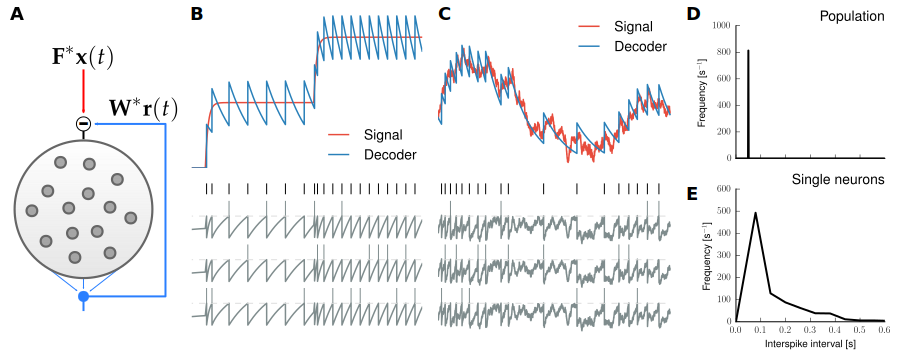
\includegraphics[width=\textwidth]{../plots/Fig1.pdf}
  \caption{Encoding of a one-dimensional signal in a three-neuron network. \textbf{(A)} Schematic of optimal balanced networks. Steady-state membrane potentials of the neurons in the network receive balanced input from the encoding $\b{F}^*\b{x}(t)$ and decoding signal $\b{W}^*\b{r}(t)$. Thus, membrane potentials represent prediction errors of the reconstructed signal. \textbf{(B)} Step function (red) and decoding signal (blue) in a single trial. The membrane potential and spike trains for each of the three neurons are shown in separate colors and rows. \textbf{(C)} Random signal as input, otherwise same as \textbf{(B)}. Note the trade-off between decoding accuracy and overall numbers of spikes emitted. \textbf{(D}--\textbf{E)} Interspike interval (ISI) distribution for population \textbf{(D)} and single-neuron \textbf{(E)} spike trains.}
  \label{fig:1Dsys}
\end{figure*} 

In order to describe the time-varying membrane potential $\b{V}(t)$, we take its temporal derivative
\begin{align}
\tau \dot{\b{V}}(t) &= \tau (\b{F}\dot{\b{x}}(t) - \b{W} \dot{\b{r}}(t)) \nonumber \\
&= -\b{F}(\b{x}(t)-\b{c}(t)) + \b{W} (\b{r}(t)-\b{o}(t)) \nonumber \\
&=  -(\b{F}\b{x}(t) - \b{W}\b{r}(t)) + \b{F}\b{c}(t) - \b{W}\b{o}(t)  \nonumber \\
&= -\b{V}(t) + \b{F}\b{c}(t) - \b{W}\b{o}(t), \label{eqn:lifneuron}
\end{align}
using Eqn. (\ref{eqn:voltage}) for the membrane potential. Therefore, we derived a network model equivalent to leaky integrate-and-fire neurons \cite{Stein1967} with threshold $\Theta$ and reset $2\Theta$. Given that the loss function is minimized, membrane potentials fluctuate around zero, and therefore the balance of excitatory and inhibitory currents of $\b{F}\b{c}(t)$ and $\b{W}\b{o}(t)$, respectively. In Fig. \ref{fig:1Dsys}, we illustrate the network dynamics in a three-neuron example encoding a one-dimensional signal. While single neuron spike trains exhibit poisson-like statistics (Fig. \ref{fig:1Dsys}D), the overall spiking of the population is regular given a constant input (Fig. \ref{fig:1Dsys}E).

 \subsection{Learning of recurrent connectivity}
 
 How can a randomly connected network learn to form optimal recurrent connections? From the leaky integrate-and-fire dynamics in Eqn. \ref{eqn:lifneuron}, we recall that an optimal connectivity achieves the balance of excitation and inhibition. For steady-state, optimal solutions, the membrane potentials $\b{V}(t)$ will fluctuate around zero:
\begin{align}
0 = \langle \b{V}(t) \rangle = \dot{\b{r}}(t) - \b{V}(t).
\end{align}

A spike from neuron $i$ at time $t_k$ will reduce the membrane potential by $\b{W}\b{e}_i$, so that 
\begin{align}
\b{V}(t_k) \rightarrow \b{V}(t_k) - \b{W}\b{e}_i. 
\end{align}
For a tight balance (i.e., $\langle \b{V}(t) \rangle = 0$), we demand the steady-state equality
\begin{align}
(\b{W}\b{e}_i)_\infty = -2\b{V}(t_k)
\end{align}
which can be formed by a linear differential equation given by
 \begin{align}
 \frac{1}{\eta}  \dot{\b{W}}_i =  2\b{V}(t) - \b{W}_i, \hspace{0.5cm} \textnormal{if }i \textnormal{ spikes,}
 \end{align}
 where $\b{W}_i \equiv \b{W}\b{e}_i$ and $\eta$ is a constant learning rate. This is the voltage-based learning rule without the quadratic cost term. 
 
Considering the cost term, each spike by neuron $i$ leads to $\b{V}(t_k) \rightarrow \b{V}(t_k) - \b{W}\b{e}_i  - \mu \b{e}_i$. Tight balance is achieved for the steady state, if
\begin{align}
\b{W}_i = \b{F}\b{D}_i +\mu \b{e}_i
\label{eqn:learn}
\end{align}
Therefore, we construct a learning rule based on a linear differential equation given by
  \begin{align}
 \frac{1}{\eta} \dot{\b{W}}_i = 2(\b{V}(t)+\mu \b{r}(t)) - \b{W}_i + \mu \b{e}_i,
 \label{eqn:learncost}
 \end{align}
 if neuron $i$ spikes.
%------------------------------------------------

\section{Simulations}
\label{sec:results}

\begin{figure*}[!ht]
  \includegraphics[width=\textwidth]{../plots/Fig2.pdf}
  \caption{Encoding of a two-dimensional, circular signal in a network of $N=16$ neurons using a quadratic cost factor of $\mu=0.1$. \textbf{(A)} Input signal $\b{x}(t)$ and decoding signal $\b{y}(t)$ for $T=10$ ~s. After only a few time steps, the coding error $\|(\b{x}(t)-\b{y}(t) \|^2$ between input and decoder is bounded by $\Theta=\frac{\|\b{D}\|}{2}$. \textbf{(B)} Feed-forward encoding and decoding weight vectors $(\b{F}^T)_i$ and $\b{D}_i$, respectively, in signal space. The edgecolor of the encoding vectors are black, while the decoding vectors are indicated by a gray edgecolor. Each neuron is color-coded using the Matplotlib colormap \textsc{''winter''}. The same color code is used in \textbf{(C}--\textbf{D)}.  \textbf{(C)} Spike raster and firing rates for simulating the network for $T=30$ s. The spike pattern reflects the periodic nature of the incoming signal. The population rate $R(t) = \frac{\sum_i^Nr_i(t)}{N}$ is indicated by the black solid line. Note that, while single neuron spiking is variable, the population rate is reliably constant and is proportional to the amplitude of the input signal. \textbf{(D)} Numerical estimation of tuning curves of the network using univariate spline interpolation of firing rates over $T=500$~s. }
  \label{fig:2Dsys}
\end{figure*}

In order to examine the interactions between optimal balanced compensation and recurrent plasticity during neuronal death, we carried out numerical simulations of optimal balanced networks with $N=16$ neurons encoding a two-dimensional signal $\b{x}(t)$ given by
\begin{align}
\b{x}(t) = \begin{pmatrix}
5\cos(t) \\
5\sin(t)
\end{pmatrix},
\end{align}
which describes a circle in the two-dimensional space.
The differential equations from section \ref{sec:derive} are numerically solved using linear Euler integration $x(t+dt)=x(t)+dt\cdot\dot{x}(t)$. Therefore, spike trains have to be scaled by $\frac{1}{dt}$ in order to mathematically be equivalent to a delta distribution as defined above. For all simulation described in this report, we applied an integration step size of $dt = 0.001$. Since this is approximately the time scale of spikes ($\approx 1$ ms), we have all temporal variables defined in seconds (s). Note that spike rates therefore are described in Hertz (Hz). All other variables are assigned with arbitrary units, but it is possible to assign physical units by applying appropriate scalings and offsets. The time constants of the differential equations are set to $\tau=1$ s. Note that individual time scales can be applied for model fitting. 

Fig.~\ref{fig:2Dsys} shows the results of an optimal network with 16 neurons encoding $\b{x}(t)$ for a total duration of $T=30$ s. Fig.~\ref{fig:2Dsys}A shows the signal $\b{x}(t)$ and the decoder readout $\b{y}(t)$ for the first ten seconds of the simulation, showing that the accurate representation of the signal is achieved rapidly by fast, repeated spiking. Almost instantaneously the membrane potential is bounded and balanced between $-\Theta$ and $\Theta$, effectively bounding $\b{y}$ around $\b{x}$ by $\frac{\|D\|}{2}$. Fig.~\ref{fig:2Dsys}B shows the 16 encoding vectors  $(\b{F}^T)_i$ and decoding vectors $\b{D}_i$ in the signal space. The weights are set to 
\begin{align}
(\b{F}^T)_i = \b{D}_i  = \begin{pmatrix}
\cos(2\pi i) \\
\sin(2\pi i)
\end{pmatrix},  i \in [0, N-1]
\end{align}
which is shown by the exact alignment and evenly spaced vectors. Furthermore, tight balance in the network is achieved for the case of $\b{W}=\b{F}\b{D} - \mu \mathbb{1}^N$. In this simulation, we applied a quadratic cost factor of $\mu=0.1$, which increases self-inhibition and therefore reduces firing rates. In Fig.~\ref{fig:2Dsys}C, spike raster and firing rates are shown, where the population rate $R(t) = \frac{\sum_i^Nr_i(t)}{N}$ is indicated by the black solid line. The spike pattern describes population-wide the oscillatory course of the encoded signal, while individual spikes are variable. The tuning curves of each neuron is shown in Fig.~\ref{fig:2Dsys}D, which describe bell-shaped function similar to the orientation tuning in the visual cortex or directional tuning in the cricket cercal system. Note that the tuning curves have been calculated numerically from a longer simulation ($T=500$ s). Therefore, we can explain the long tails in the curves by the way we estimate the rates using an exponential kernel.

\begin{figure}[!ht]
  \includegraphics[width=\columnwidth]{../plots/Fig3.pdf}
  \caption{Effects of different quadratic cost factors $\mu$ on mean population firing rates, their variances, and mean squared coding errors. We varied $\mu$ with values $0.0$, $0.01$, $0.02$, $0.1$, $0.2$, $0.5$, $1$, $2$, $5$, $10$, which are individually color-coded. The gray solid line indicates the mean values for each value of $\mu$.}
  \label{fig:mu}
\end{figure}

In order to measure the effect of different quadratic cost factor $\mu$ on the firing statistics and coding accuracy, we carried out ten simulations ($T=100$ s) for each of the values $\mu = \{ 0.0, 0.01, 0.02, 0.1, 0.2, 0.5, 1, 2, 5, 10 \}$. We measured for each of the simulation the mean population rate $\langle R(t)\rangle$, mean population rate variance $\sigma^2_R$, and mean squared coding errors $\langle \epsilon \rangle = \langle \| \b{x}-\b{y} \|^2 \rangle$. Note that the mean is calculated across time of individual trials. The results are shown in Fig. \ref{fig:mu}, where the mean of the ten repetitions of each value for $\mu$ is indicated by the dark-gray colored solid line.



\subsection{Learning optimal recurrent weights}

 \begin{figure*}[!ht]
  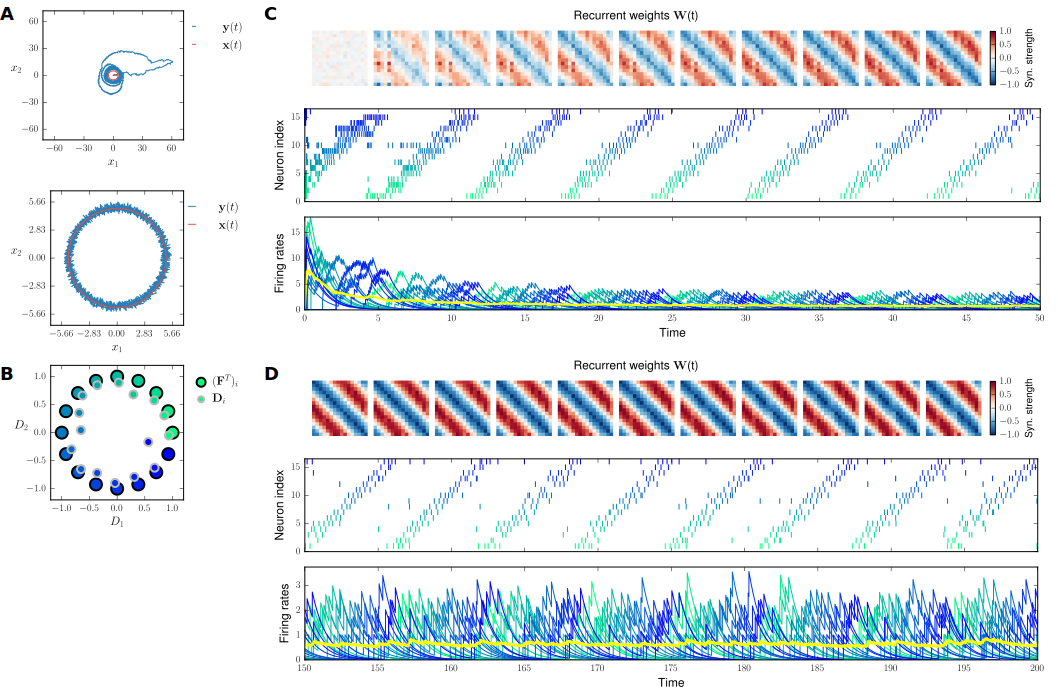
\includegraphics[width=\textwidth]{../plots/Fig4.pdf}
  \caption{Learning optimal recurrent connectivity in a network of $N=16$ neurons using a quadratic cost factor of $\mu=0.01$. \textbf{(A)} Input signal $\b{x}(t)$ and decoding signal $\b{y}(t)$ during the initial phase of learning at $t=0 - 50$~s (top) and final phase of learning at $t = 150-200$~s (bottom). First, the decoder is overshooting the signal reflecting suboptimal recurrent weights, which favor excitation in the network. After learning, the coding error is bounded like in the optimal network in Fig.~\ref{fig:2Dsys}. \textbf{(B)} Feed-forward encoding and decoding weight vectors $(\b{F}^T)_i$ and $\b{D}_i$, respectively, in signal space. The edgecolor of the encoding vectors are black, while the decoding vectors are indicated by a gray edgecolor. We used the same color code as in Fig. \ref{fig:2Dsys}. \textbf{(C}--\textbf{D)} Recurrent weight matrix, spike trains and firing rates with respect to time for \textbf{(C)} $t=0-50$ s and \textbf{(D)} $t=450-500$ s. The population rate is shown as a yellow solid line.}
  \label{fig:Learn}
\end{figure*}

In order to show that Eqns.~\ref{eqn:learn} \& \ref{eqn:learncost} lead to stable convergence of $\b{W}(t)$ towards optimal recurrent weights $\b{W}^*=\b{F}\b{D} + \mu \mathbb{1}^N$, we carried out a simulation for $T=200$ s with a learning rate of $\eta=0.01$. The results are shown in Fig.~\ref{fig:Learn}. We initialize the recurrent weight matrix as a Gaussian random matrix, where each entry is drawn from a Gaussian distribution.  
\begin{align}
W_{ij} \sim \mathcal{N}\left(0,\frac{1}{N^2}\right).
\end{align}
The encoding weight vectors $(\b{F}^T)_i$ are assumed to be fixed and optimal for the circular input signal as described above. The decoding weight matrix $\b{D}$ is calculated from the final recurrent weights using
\begin{align*}
\b{W}(T) &\approx \b{F}\b{D} \\
\Leftrightarrow \b{D} &\approx \b{F}^+\b{W}(T),
\label{eqn:pseudo}
\end{align*}
where $\b{F}^+$ is the Moore-Penrose inverse matrix of the encoding weights. Fig.~\ref{fig:Learn}A shows the input and decoder signal for the first (top) and final 50 (bottom) seconds, respectively. After learning, the decoder reconstructs the input signal accurately up to $\frac{\|\b{D}\|}{2}$. In Fig.~\ref{fig:Learn}B, the encoding and decoding weight vectors are shown. Since the cost factor $\mu=0.01$ is relatively small, the optimal solution for the firing rates allow for additional firing, which are indicated by near-optimal recurrent and therefore also decoding weights. Fig.~\ref{fig:Learn}C \& D shows the time evolution of recurrent weights $\b{W}(t)$, spike trains, and firing rates for the first (C) and the final (D) 50 seconds. During learning, the recurrent weights approach towards the optimal solution, which reduce the firing rates given by the unbalanced, random initial weights. Note that the population rate is shown as a yellow solid line. After learning, the spike pattern exhibits are similar periodic spike pattern and constant-mean fluactuating firing rate as in Fig.~\ref{fig:2Dsys}.

\subsection{Optimal balance and recurrent plasticity for compensating neuronal death at constant rate}

 \begin{figure*}[!ht]
  \includegraphics[width=\textwidth]{../plots/Fig5.pdf}
  \caption{Comparison of networks with and without recurrent plasticity during constant-rate neuronal death. \textbf{(A}--\textbf{B)} Input signal $\b{x}(t)$ and decoding signal $\b{y}(t)$ during the final $50$ s, as well as the final encoding and decoding weight vectors for the \textbf{(A)} plastic and \textbf{(B)} static network. The color code is similar to the previous figures. \textbf{(C)} Recurrent weight matrix with respect to time. The time difference between each display is $\Delta t = 100$ s to show effects of individual ablations. \textbf{(D)} Coding distance and population rates for the plastic and static network. We measure coding accuracy by using the distance $\|\b{x}-\b{y}\|$ between input and decoding signal, which is lower for the plastic network (i.e., better coding accuracy). We show that recurrent plasticity reduces the variance of the population rate by equalizing the increase of certain firing rates due to acute optimal balance compensation.}
  \label{fig:recovery}
\end{figure*}

We carried out several simulations with a network described in the section above for $T=2000$ s, in which we ablate neurons sequentially in random order. An ablation of neuron $i$ at $t_{\textnormal{abl},i}$ is given by setting
\begin{align}
\b{F}^T_i (t) = \b{W}_i (t)= \b{W}^T_i(t) = V_i (t) = 0, \nonumber\\
 \forall t \in [t_{\textnormal{abl},i},T]. 
\end{align} 
Ablations are at a constant rate of $f_{\textnormal{abl}}=0.01$~s$^{-1}$ (i.e., one ablation per $100$~s) and start after an initial phase of $10$ seconds, so that the network is not driven by transients. We initialize optimal recurrent weights $\b{W}=\b{F}\b{F}^T$. All other parameters are defined as described above. We compare a network with recurrent plasticity to one with static connectivity. Since the feed-forward and recurrent weights are changed with each ablation, we constantly recalculate the decoding matrix $\b{D}$ using the pseudoinverse relation from Eqn. \ref{eqn:pseudo}. 

Fig. \ref{fig:recovery} shows the results of comparing the plastic and the static network during neuronal death. The order of neurons that are ablated is random, but same for both networks: $\{ 0, 1, 5 ,14,13,11, 8,9,2,15\}$. After these ten ablations ($\cong62.5$ \% of the population), the network is further simulated until it reaches $t=T$. Fig. \ref{fig:recovery}A \& B show the signal (input and decoder) and weight space (feed-forward and decoding) of the plastic (A) and static (B) network of the final 50 seconds, respectively. While the static network has a decreased coding accuracy for the lower right quadrant of the input signal, the plastic network adapts its recurrent weights to compensate for this error. Fig. \ref{fig:recovery}C shows the recurrent connectivity of the plastic network with respect to time. Note that each matrix are spaced in time by $\Delta t=100$ s, in order to show individual ablations. It is apparent, that the amplitude of recurrent weights is decreased as neurons are ablated. Fig.~\ref{fig:recovery}D shows the functional consequences of recurrent plasticity in terms of coding. We measured the coding distance $\|\b{x}-\b{y}\|$ and show that the plastic network has a distance below $1$ for most of the time. The static network shows periodically high coding inaccuracies corresponding to the ablated neurons. Furthermore, the firing rates of both networks increase as neurons are ablated. However, the plastic network exhibits a lower variance of the population rates. It shows that in the plastic network, the increase of firing rates is homogenous across the population.


\section{Conclusions}
\label{sec:discuss}

In summary, we showed that optimal balanced networks do not only offer acute compensation for neuronal death, but when combined with learning rules, it further restores balance of excitation and inhibition. This is due to a decrease in population rate variance. For future work, it would be interesting to include feed-forward plasticity \cite{Brendel2016}, because this way the network could be perturbed to the theoretical limit of possible ablations without losing coding accuracy (see Appendix). Furthermore, the network could be fed by a higher-dimensional signals, which are usually given in sensory systems. Nonetheless, this project was an important step towards understanding interactions of neuronal and synaptic compensations during neuronal death.

%----------------------------------------------------------------------------------------
%	REFERENCE LIST
%----------------------------------------------------------------------------------------
%\clearpage 
 \bibliography{report}

%----------------------------------------------------------------------------------------
\clearpage
\section*{Appendix}

\subsection*{Geometry of a spike}
\begin{figure*}[!ht]
\centering
  \includegraphics[width=\textwidth]{../plots/2simplex.pdf}
  \caption{Examples of (A-B) bounded and (C-D) unbounded error conditions for the 3-neuron network in two dimensions.}
  \label{fig:N3}
\end{figure*}

In the last section, we defined the spike mechanism of a neuron as a form of loss reduction for a given error and cost. Since $\b{x}$, $\b{y}$ and $\b{D}_i$ lie in the same vector space $\R^M$, we are able to apply geometry to understand, when a spike is triggered and how a spike affects the loss function. In order to simplify this analysis, we neglect the cost term $C(\b{r}(t))$ for now. Thus, we examine the trajectory of the error $\boldsymbol{\epsilon}(t) = \b{x}(t)-\b{y}(t)$, for which the spiking mechanism in Eqn. (\ref{eqn:spiking}) can be rewritten as
\begin{align}
\b{D}^T_i\boldsymbol{\epsilon}(t) > \frac{\b{D}^T_i\b{D}_i}{2},
\end{align}
where $\b{D}^T_i\b{D}_i=\| \b{D}_i \|^2=\| \b{D}^T_i \|^2$ is the squared vector norm of $\b{D}_i$. This leads to
\begin{align}
\frac{\b{D}^T_i}{\| \b{D}^T_i \|}\boldsymbol{\epsilon}(t) > \frac{\| \b{D}_i \|}{2},
\label{eqn:project}
\end{align} 
and therefore neuron $i$ spikes, when the scalar projection of the error $\boldsymbol{\epsilon}(t)$ onto the weight vector $\b{D}_i$ exceeds more than half of its vector length in the signal space $\R^M$. Therefore, the spiking thresholds $\Theta_i$ can be seen as hyperplanes 
\begin{align}
\mathcal{H}_i = \left\{ \b{v} : \b{D}_i^T\b{v} = \frac{\Theta_i}{\|\b{D}_i \|}\right\}
\end{align} 
spanning in $\R^M$. As neuron $i$ elicits a spike, we recall that $\b{y}$ increases by $\b{D}_i$, and thus $\boldsymbol{\epsilon} \rightarrow \boldsymbol{\epsilon} - \b{D}_i$ that moves $\boldsymbol{\epsilon}(t)$ inside the threshold boundary. The intersections of hyperplanes $\{\mathcal{H}_i\}_{i=1}^N$ which form a so-called \textit{polytope}, a convex hull of a bounded, finite set of points. This is given, if $N\geq M+1$, and $\left| \frac{\b{D}^T_i\b{D}_j}{\|\b{D}_i \|\|\b{D}_j \|}\right| < 1 \hspace{0.5cm} \forall i \land  (j \neq i)$ for the special case of $N=M+1$, . The error $\boldsymbol{\epsilon}(t)$ is bounded for $t\rightarrow\infty$, if and only if the polytope of hyperplane intersections contains the origin $\b{0}$, where the squared error is zero.

\subsubsection*{Examples in two dimensions}

Here, we illustrate two simple examples in a low-dimensional ($M=2$) space. Using these examples, we aim to describe spiking properties of the network for error boundedness and convexity.

\paragraph*{Example 1: $N=3$ (2-simplex)\\}

In two dimensions, the minimum number of neurons in order to bound the error is $N=3$. In this extreme case, we also demand that all pairs of threshold boundaries are not parallel to each other. In Fig. \ref{fig:N3}, we show examples of different sets of decoding vectors and their resulting thresholds boundaries. In the leftmost case, the decoding vectors are span in $\R^2$ evenly with equal length. We then varied the angle $\alpha_{\b{D}_0}$ to the x-axis increasing it by $30^\circ$ each time, while keeping the other vectors constant. The red-colored area indicates the polygon formed by the intersections of the threshold boundaries. For $\alpha_{\b{D}_0} = 0^{\circ}$ and $30^\circ$, the polygon contains the origin, and therefore the error $\boldsymbol{\epsilon}$ is bounded. For $\alpha_{\b{D}_0} =90^{\circ}$, two of the threshold boundaries are parallel, such that the error cannot be bounded. As the vector is further rotated, the polygon of the intersection does not contain the origin, and therefore error boundedness is not given. Note that it is equivalent to say that the error is bounded, if the vector span of the decoding vectors is equal to $\R^N$. 

As described above, each spike leads to $\boldsymbol{\epsilon}\rightarrow\boldsymbol{\epsilon}-\b{D}_i$, which may lead to an error outside another threshild boundary under certain conditions. Therefore the network would elicit multiple spikes in consecutive time steps. The 3-neuron network is a special case, where multispiking occurs very likely. In Fig. \ref{fig:multispike}, we illustrate this phenomenon by several examples.    

\begin{figure*}[!ht]
\centering
  \includegraphics[width=\textwidth]{../plots/doublespike.pdf}
  \caption{Examples of multiple spikes in the 3-neuron network for two dimensions. Depending on a given error, the neuron can spike (A) one, (B) two, or (C) more times to reach inside the error bound. (D) Assuming that the error dynamics are slow, i.e., the error slowly reaches the threshold, one can illustrate possible effects of a spike by a rectangle spanned by $-\b{D}_i$. The probability of exhibiting two spikes is therefore given by the ratio of areas outside vs. inside the error bound.}
  \label{fig:multispike}
\end{figure*} 
 
%\paragraph*{Example 2: $N > 3$\\} 
 
%For four neurons (Fig. \ref{fig:N4}), the error bound is generally given by a quadrilateral. If the readout vectors $\b{D}_i$ are given by pairs of orthogonal vectors, the error is bounded in such a way, that multispiking for slowly-varying inputs does not occur (Fig. \ref{fig:N4}A). When threshold boundaries overlap (Fig. \ref{fig:N4}B), certain decoding weights are redundant and effectively reduces the four-neuron case to three neurons. Finally, multiple spikes can also occur for four neurons, if the pairs of parallel threshold boundaries are not orthogonal to each other (Fig. \ref{fig:N4}C).
 
 
%\begin{figure*}[!ht]
%\centering
 % \includegraphics[width=0.64\textwidth]{../plots/rect.pdf}
 % \caption{Examples of error bounds in the four-neuron network for two dimensions.}
 % \label{fig:N4}
%\end{figure*} 

%\begin{figure}[!ht]
%\centering
 % \includegraphics[width=0.64\columnwidth]{../plots/5.pdf}
%  \caption{Examples of bounded and unbounded error conditions for the 3-neuron network in two dimensions.}
 % \label{fig:N5}
%\end{figure} 
 
 
\end{document}
